Em química analítica, é possível determinar satisfatoriamente a concentração de metais em solução usando
agentes complexantes. O agente quelante mais utilizado é o EDTA, visto que ele reage com os cátions
metálicos em uma proporção bem definida de $1:1$. O EDTA é um ácido poliprótico com quatro prótons
ionizáveis, cuja estrutura pode ser simplificada pela fórmula \chemfig{H_4Y}. Titulações com EDTA são feitas
comumente em soluções tamponadas de pH = 10, para que não haja competição entre os íons metálicos e os
íons \chemfig{H^+}, garantindo a formação de um complexo estável.
Uma das grandes utilidades do uso de EDTA é para a determinação de cálcio e magnésio.
As reações de complexação e suas respectivas constantes de equilíbrio são apresentadas abaixo.

\begin{center}
	\schemestart
	\chemfig{Mg^{2+}{(aq)}} + \chemfig{Y^{4-}{(aq)}} \arrow{<=>} \chemfig{MgY^{-2}{(aq)}} \qquad \qquad $K_f = 4,9 \times 10^{8}$
	\schemestop

	\schemestart
	\chemfig{Ca^{2+}{(aq)}} + \chemfig{Y^{4-}{(aq)}} \arrow{<=>} \chemfig{CaY^{-2}{(aq)}} \qquad \qquad $K_f = 5,0 \times 10^{10}$
	\schemestop
\end{center}

No processo de titulação é utilizado o indicador negro de Ericromo T (\chemfig{H_3In} em sua forma protonada), que forma complexos de cor vermelho-vinho com os metais em solução.
Em pH = 10, quando deslocado pelo EDTA, o indicador encontra-se na forma \chemfig{HIn} -- de cor azul.
Logo, o final da titulação é tido quando a solução assume uma coloração azul indicando o excesso do indicador livre.
O gráfico para a titulação complexométrica de cálcio e magnésio, em pH = 10, é apresentado a seguir.

\begin{center}
	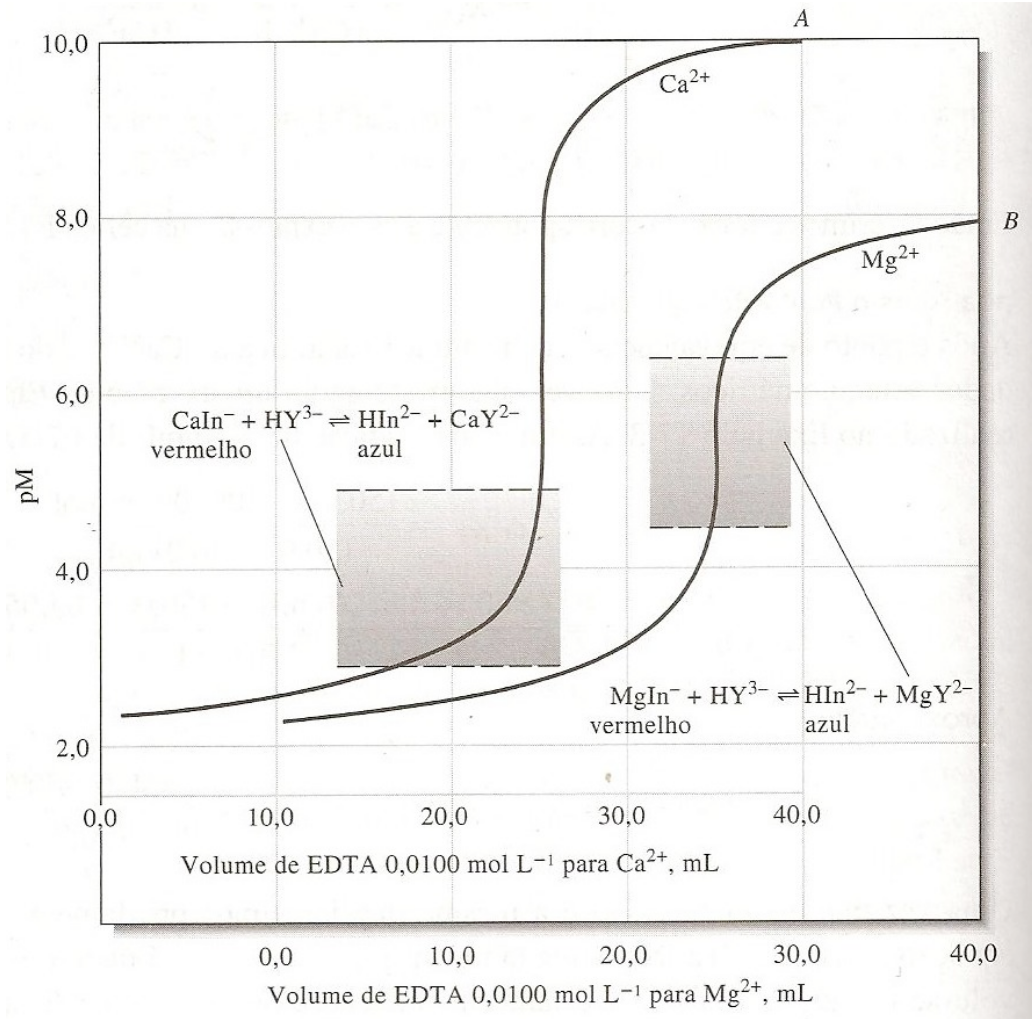
\includegraphics[width=0.5\textwidth]{figure.png}
\end{center}

Para se determinar a concentração de uma solução de \chemfig{Ca^{2+}}, foi preparada uma solução de EDTA dissolvendo \chemfig{Na_2H_2Y}.
\chemfig{H_2O} em água e completando o volume do balão até 250 mL.
Como a concentração de EDTA era desconhecida, foi usada uma solução de \chemfig{Mg^{2+}} de concentração 0,0050 M para padronização.
O volume gasto na padronização de 25,0 mL da solução de EDTA foi de 18,5 mL da solução de \chemfig{Mg^{2+}}.
Antes de iniciar a titulação da solução cálcio, 50,0 mL dessa solução foram misturados com 50,0 mL da solução de magnésio utilizada na padronização do EDTA.
A nova solução foi diluída em balão volumétrica até o volume de 500 mL.
Uma alíquota de 50 mL foi então tamponada em pH = 10 e titulada com a solução de EDTA gastando 9,7 mL para que a solução ficasse azul.

\begin{enumerate}[label = (\alph*)]
	\item Explique analiticamente o porquê da adição de magnésio à solução de cálcio antes da titulação.
	\item Calcule a concentração de \chemfig{Ca^{2+}} da solução inicial. Expresse o resultado em mol$\cdot$L$^{-1}$ e em ppm.
\end{enumerate}
